\subsubsection{Subsystem Overview}
The communications subsystem consists of several network Application Programming Interface (API)
endpoints.
These endpoints cover domains such as serving camera feeds, operating a flight director which
provides continuous, real-time instructions for robot operation, creating flight plans,
and obtaining localization estimates and maps of the field.

\subsubsection{Test Plan}
There were two methods of verification which our plan called for.

The first method of verification was a comprehensive endpoint unit test suite.
Each endpoint was hit by a test client to confirm that the endpoint was showing data in the correct
format.
This was done using the unit testing facilities provided by the standard rust tooling, as well as
asynchronous HTTP clients.
Code coverage was recorded and monitored on within the communications codebase using the
Tarpaulin\cite{tarpaulin} tool to ensure that each endpoint was being hit.

The second method of verification was a manual test of network bandwidth utilization while
streaming video feeds from our cameras.
This test was conducted by starting a camera stream at 15 frames per second at a resolution of
960x540 while using Wireshark\cite{wireshark} to capture packets and plot the bandwidth usage of
the program.
The test would be successful if the bandwidth utilization was under 5,000 kilobits per second,

\subsubsection{Test Results}
The unit tests all passed after some debugging.
Ultimately, there were some initial flaws which were caught involving typos which were made in the
URL routes which resulted in messages being routed into the void, resulting in 404 messages.
After some quick debugging, these were fixed.

The bandwidth tests were also passed.
Bandwidth averaged at around 4300Kb/s.
All that mattered for this test is that bandwidth fell below our threshold, as this test served
to establish an upper band on bandwidth consumption with a high framerate and high quality images.

\begin{figure}[hbt]
    \centering
    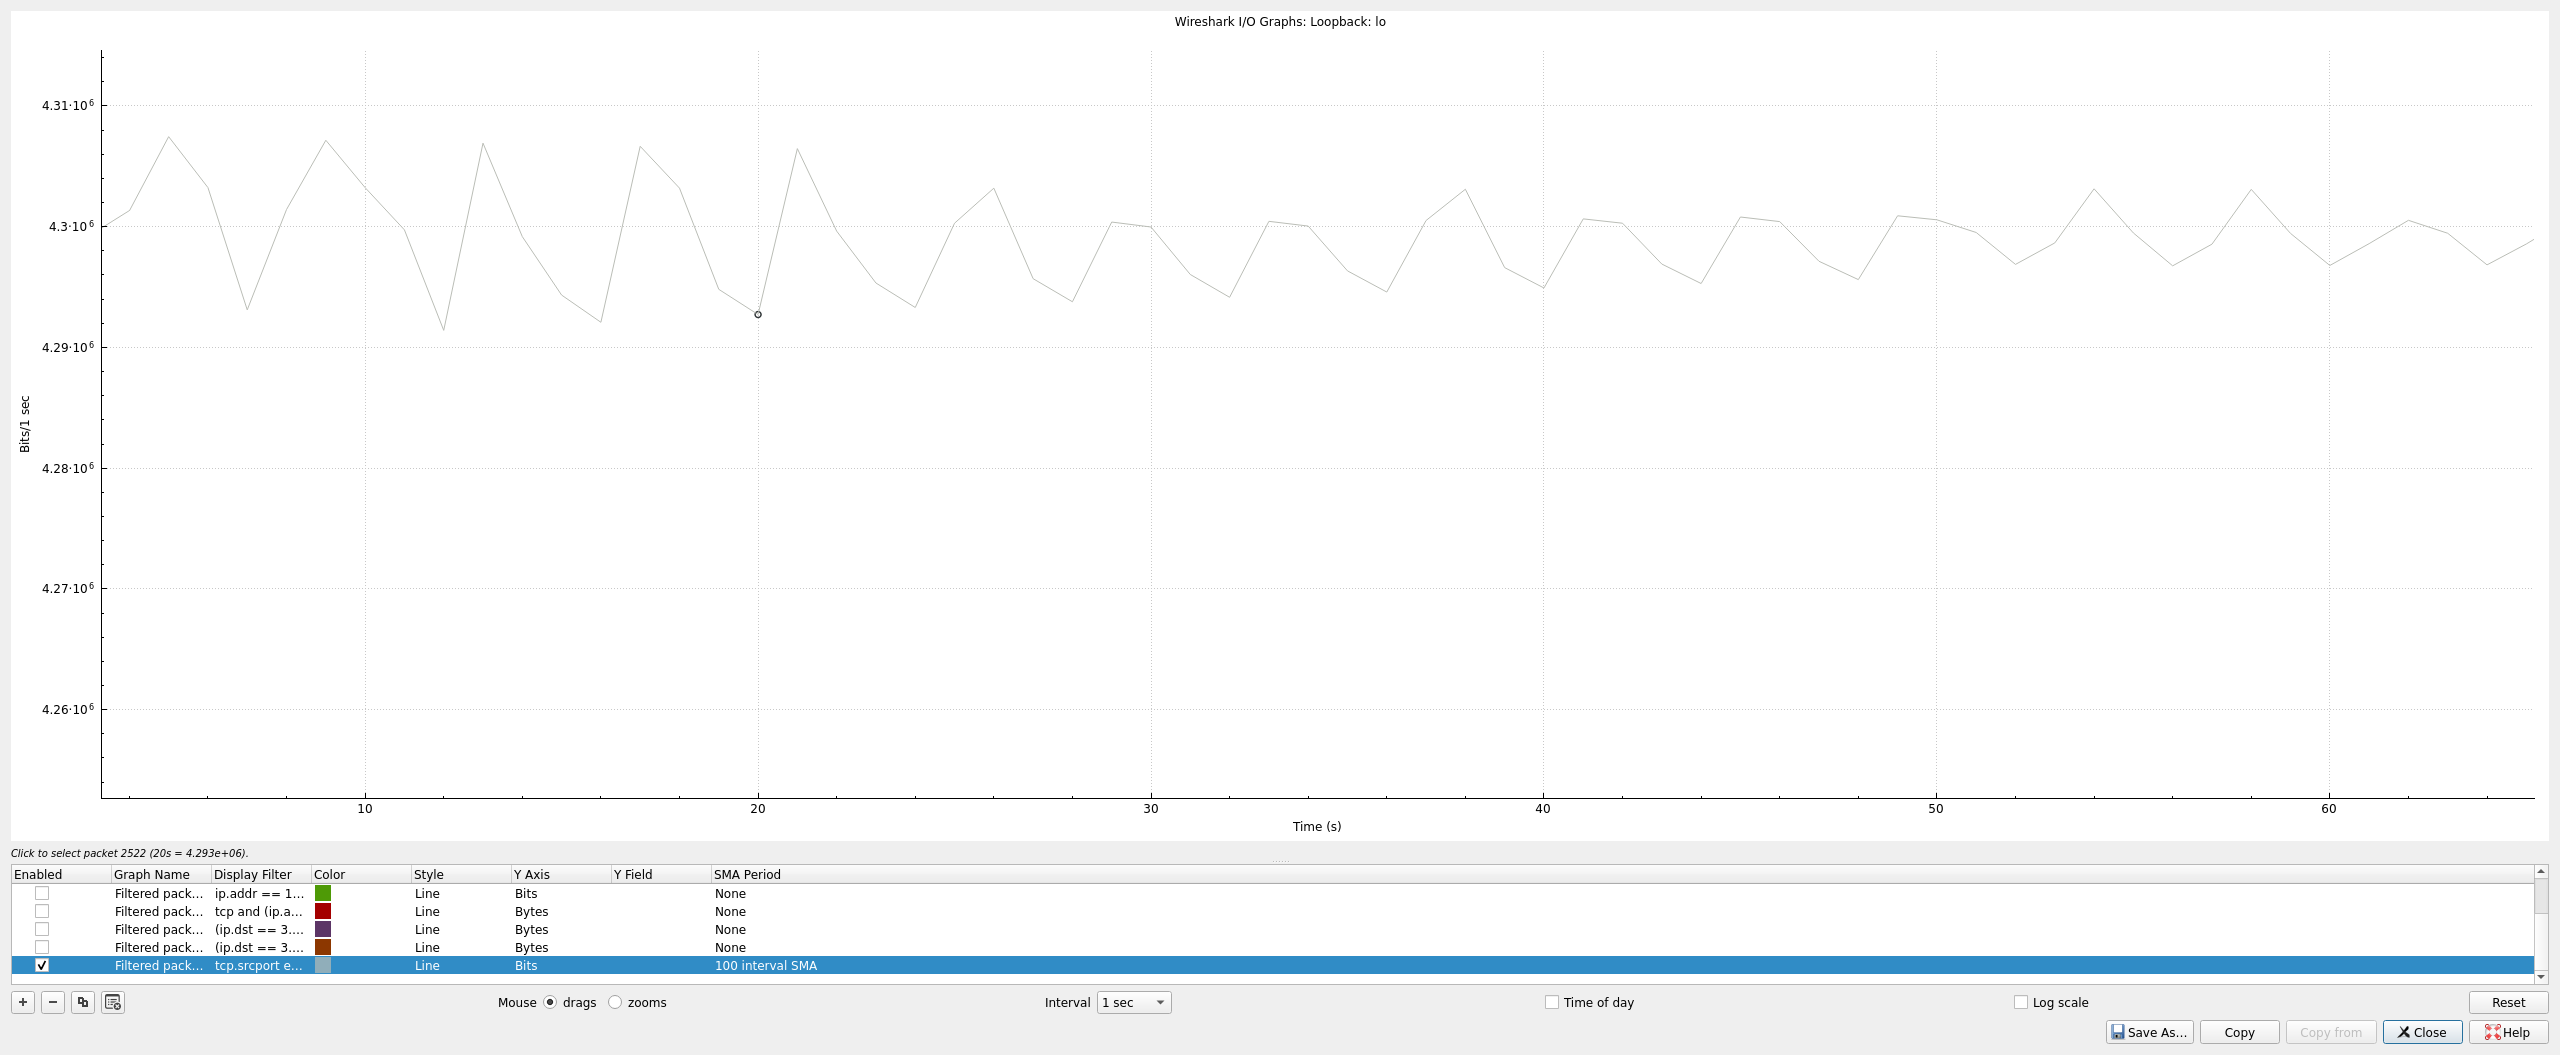
\includegraphics[width=\textwidth]{wireshark}
    \caption{
        IO Graph captured with Wireshark.
        Bandwidth remained relativel consistend throughout the run.
        A sample of eight images were used to reduce the possibility of data bias impacting our
        results.
    }\label{fig:bandwidth}
\end{figure}